% !TeX program = pdflatex
\documentclass[tikz,border=8pt]{standalone}
\usepackage{tikz}
\definecolor{FigureBlue}{HTML}{2563EB}\definecolor{FigureOrange}{HTML}{EA580C}
\begin{document}
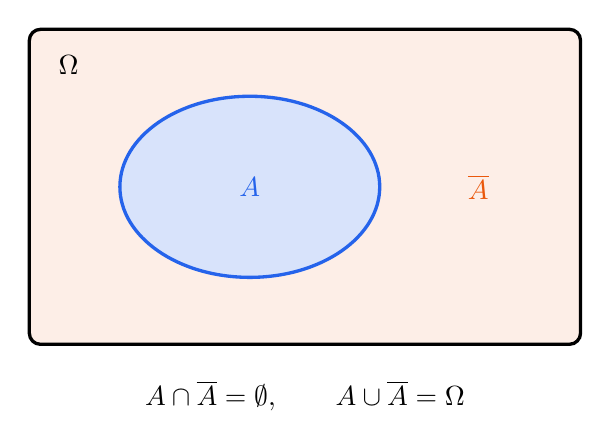
\begin{tikzpicture}
  \fill[FigureOrange!10,rounded corners] (0,0) rectangle (7,4); \draw[rounded corners,line width=1.2pt] (0,0) rectangle (7,4);
  \fill[FigureBlue!18] (2.8,2) ellipse (1.65 and 1.15); \draw[FigureBlue,line width=1.2pt] (2.8,2) ellipse (1.65 and 1.15);
  \node at (.5,3.55) {$\Omega$}; \node[FigureBlue] at (2.8,2) {$A$}; \node[FigureOrange] at (5.7,2) {$\overline A$};
  \node at (3.5,-.65) {$A\cap\overline A=\emptyset,\qquad A\cup\overline A=\Omega$};
\end{tikzpicture}
\end{document}
